% --------------------------------------------------------------------------------------
\subsection{Inclusive infrastructure}
As bicycle infrastructure is primarily publically funded, it quickly becomes a politicized topic. 
While many cities push for a \textit{build it and they will come}-approach, what is being neglected
is the need for a certain mass of cyclists to attract the casual rider and have the investment succeed.
If new cyclists feel uncomfortable (stress, embarrassment, etc.), they are more likely to give up on the bike as a viable means of everyday transportation. 
This leaves the infrastructure underutilized, with the public image of money and space being wasted, 
thus resulting in a pushback against further cycling initiatives (\cite{backlash}).
Therefore, it is important to carefully plan new cycling infrastructure and rapidly adapt to the observed behavior of new users.

 % -----------------------------------------------------------------------------------
\subsection{Previous work}

\subsubsection{Bicycle choreography}
In the study (\cite{copenhagenize2014}) an intersection in Copenhagen is reviewed, focusing on high-level aspects
such as routes taken by cyclists, as well as the behavior exhibited by the individual cyclists.
This is done by using \textit{Desire lines Analysis}, a tool pioneered by the same authors as the study (\cite{copenhagenize_book}).
\textit{Desire lines} encompass the trajectories of cyclists using both "intended pathways", usually directed through infrastructure such as
 bike lanes, but also their own paths, which may deviate from the engineered structure or legal framework.
 To assess behavior, the study splits cyclists into three groups:

\begin{itemize}
	\item \textbf{Conformists}: fully rule compliant
	\item \textbf{Momentumists}: lose interpretation of current rules. Encompasses actions legal in other countries, thus acting like a  flexible 'superset'
	\item \textbf{Recklists}: dangerous behavior - both for self and others
\end{itemize}

The proportions of cyclists belonging to each of the above groups were then compared for a day. 
Notably, the share of \textit{momentumists} increased during the afternoon.
 \ \\

A recurring observation made by the study was the tendency of cyclists to get influenced by their fellow riders. 
This behavior is described as "\textit{follow the leader}", with cyclists being more likely to imitate non-conformist 
actions when another cyclist goes first. 

\subsubsection{Staging mobilities}
The book 'Designing Mobilities' (\cite{designinig_mobilities}) explores \textit{what physical, social, technical, 
and cultural conditions contribute to the staging of contemporary urban mobilities?} 
It covers how to capture and represent \textit{mobilities} and flows by presenting a theoretical framework for 'staging mobilities'. 
Most importantly it introduces a set of concepts for articulating \textit{situational perspectives}, 
including the two metaphors \textit{the river} and \textit{the ballet}. 
 \ \\

 The \textit{river} references the notion of capturing mobility from a 'birds-eye view', including the layout, 
 flows, and obstacles of a location, and hence, can be interpreted as a 'flowing riverbed'. 
 From this perspective, we can observe road users' behavior in aggregate and as part of more significant 'streams'. 
 This can be used to encapsulate abstract and high-level features of cyclists, such as the desire lines
 when infrastructure is changed or temporary obstacles come along (e.g. road work).
 \ \\

In contrast, the \textit{ballet} is the micro-perspective, encompassing the gestures and small interactions at the individual level.
This perspective is an important supplement to the former \textit{river} as subtle interactional patterns which can, for instance,
 signal agreement or evasion.

 % -----------------------------------------------------------------------------------
\subsubsection{Case study}
\textit{Study of mobilities in 'situ'} (\cite{situ}) uses the above framework as part of a case study involving cycling infrastructure in 
Copenhagen and Amsterdam. Quantitative data (as part of the \textit{river} perspective) was obtained by filming cyclists and conducting 
"desire lines analysis" (\cite{cva}) to gain a structured overview of the behavior of cyclists and intersections. 


 % -----------------------------------------------------------------------------------
\subsection{OpenDataCam}
OpenDataCam (ODC) is an existing open-source tool for processing video footage from urban environments to quantify
traffic. The novelty of OpenDataCam comes from the simple on-site, real-time processing of video. 
\ \\

The backbone of the application is based on Darknet with YOLOv4 as the model used for detecting objects in video.
\href{https://pjreddie.com/darknet/yolo/}{YOLO}, \textit{You Only Look Once}, is a real-time object detection algorithm. 
YOLO is trained on the \href{https://cocodataset.org}{COCO dataset}, which comprises over 330,000 thousand images
with over 1,5 million objects in over 80 object classes, including cars, people and cyclists. 
It is well known for its real-time speed and accuracy (\cite{redmon2016look}). 
For OpenDataCam to run locally thus requires dedicated CUDA-enabled hardware such as an Nvidia Jetson-series device. 
\ \\

The user interacts with the application through a web interface that displays a live preview of the footage with
indicators around all detected objects.

\ \\
\raggedbottom
\noindent
\begin{tabular}{@{}cc}
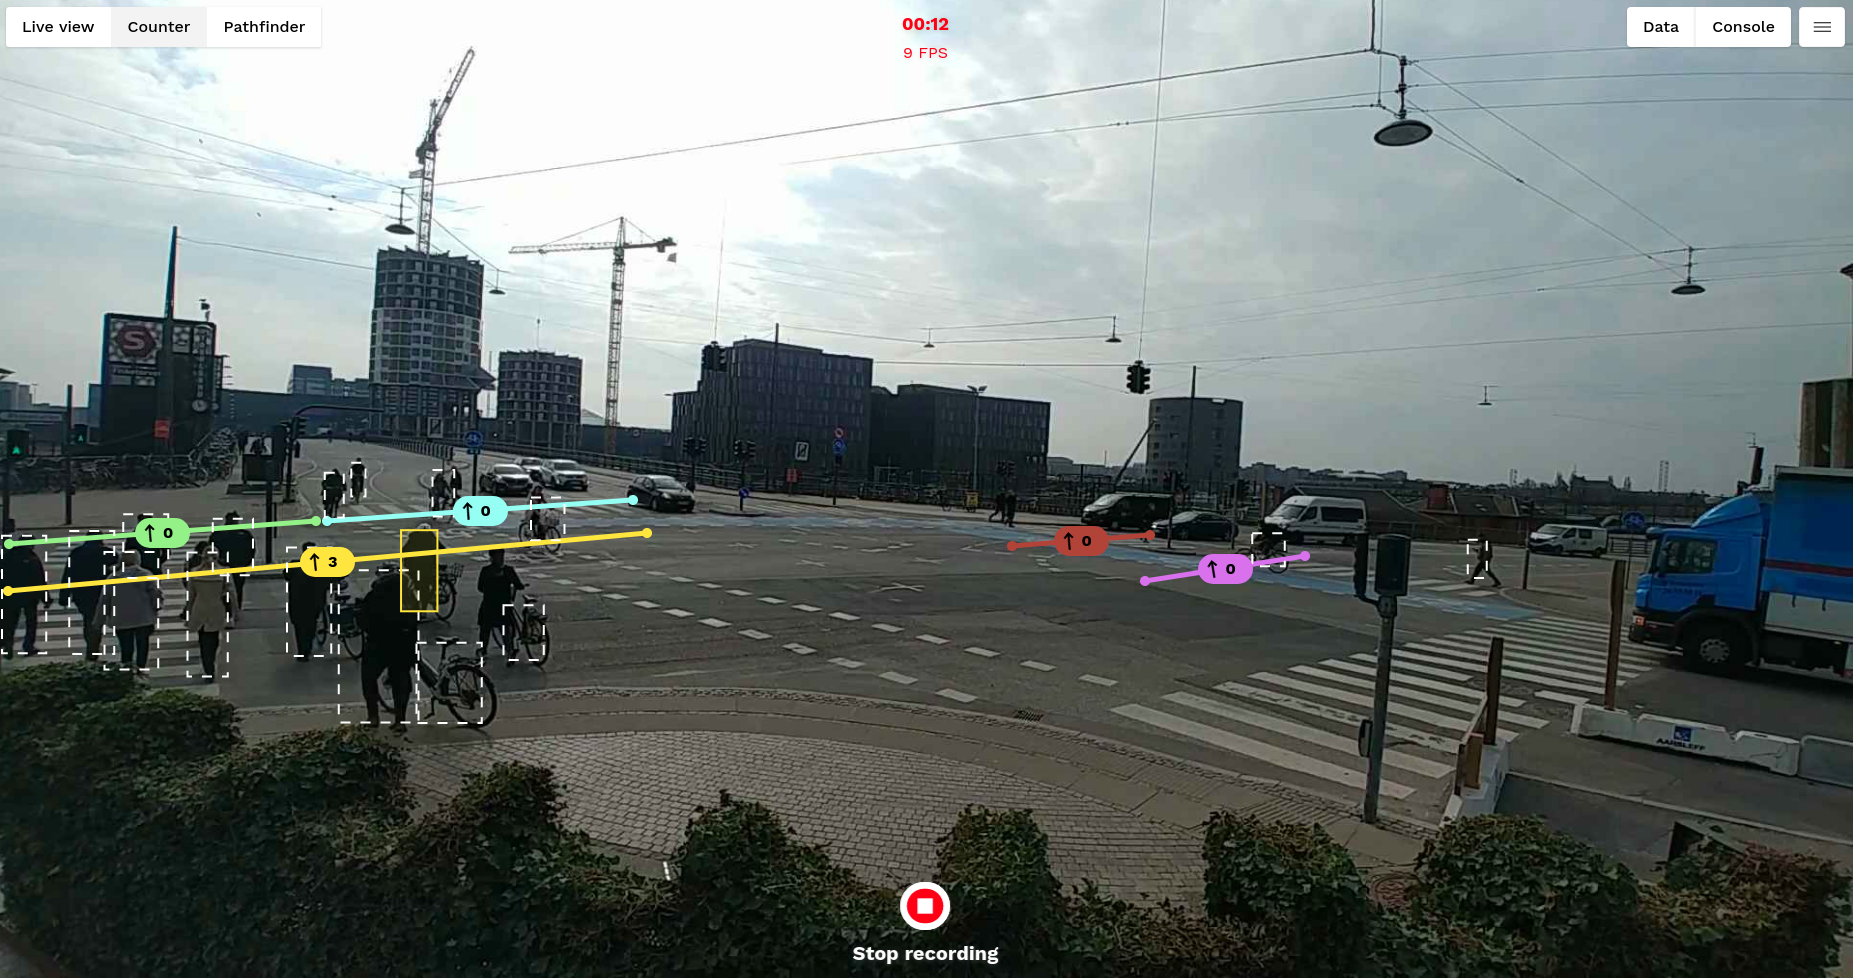
\includegraphics[width=1.0\columnwidth]{odc} 
\end{tabular}
\captionof{figure}{OpenDataCam Web Interface}
\ \\

Using the interface, a user can draw bi-directional counting lines, which, when passed by a detected object at a certain angle, 
increments a counter and keeps track of the object's identifier. Apart from counting functionality, the app also offers the trajectories of uniquely identified objects. 

\raggedbottom
\subsubsection{Application}
As a baseline, we deployed an OpenDataCam setup using pre-recorded footage from the Dybbølsbro intersection in Copenhagen.
Our setup ran on an Nvidia Jetson Xavier NX combined with two Raspberry Pis, used for filming/streaming video from the intersection.

Our goal was to extract pre-defined desire lines using the counting line functionality. We did this by drawing an initial 
'base line' followed by two (or more) additional counting lines, which would allow us to branch cyclists into multiple segments. Inspecting the
overlap of unique cyclists who passed both the base line and one (or more) of the branching lines would yield which path
they took through the intersection. 
\ \\

\ \\
\raggedbottom
\noindent
\begin{tabular}{@{}cc}
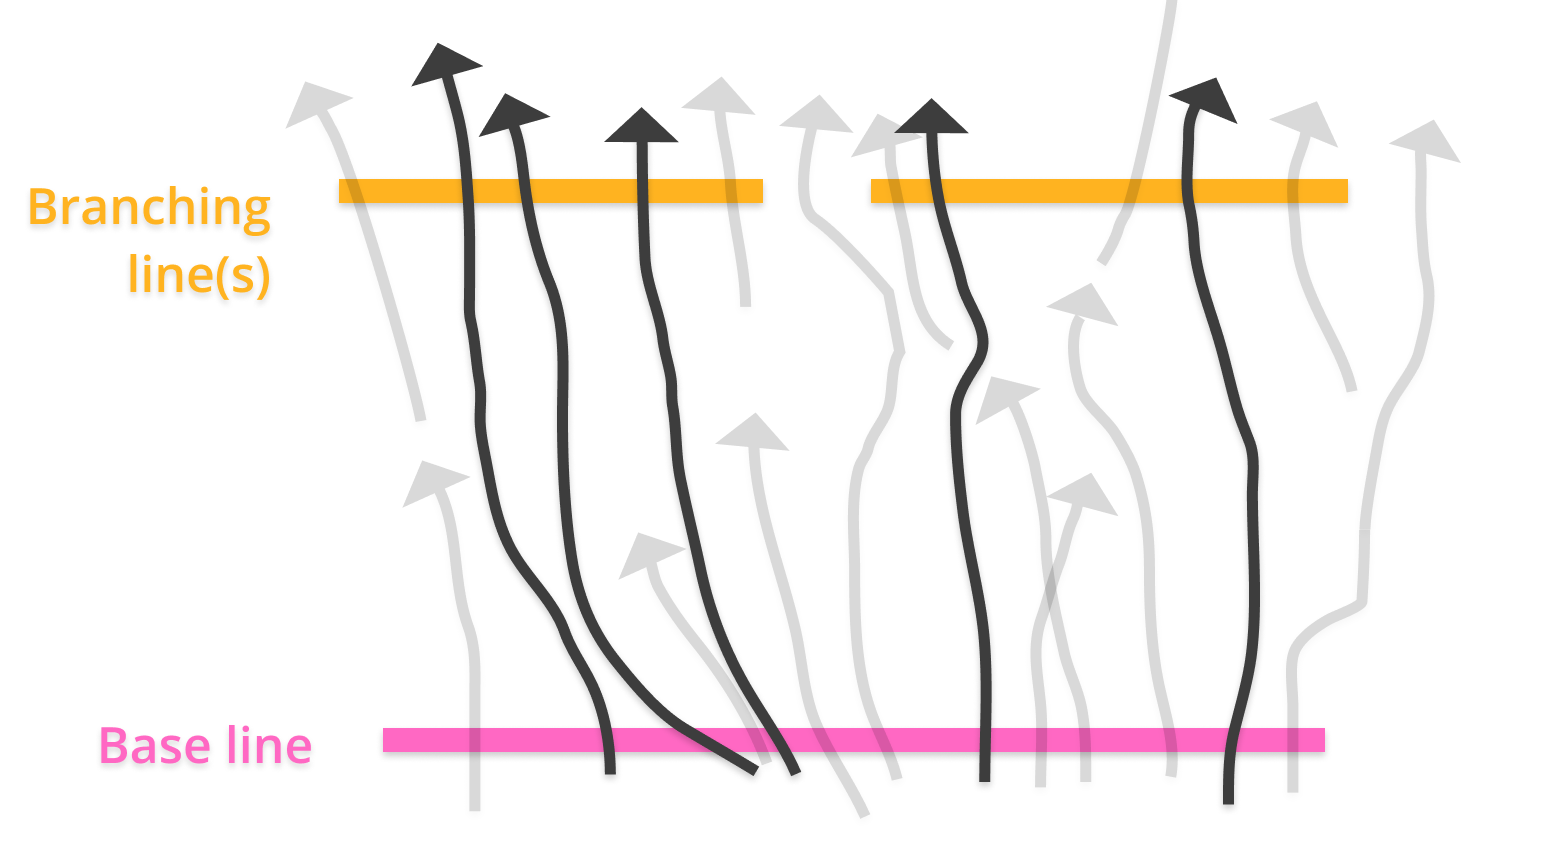
\includegraphics[width=1.0\columnwidth]{base_line} 
\end{tabular}
\captionof{figure}{'base line' (pink) and branching lines (orange)}
\ \\

However, this approach was limited by the poor performance of the detection of cyclists implemented in the current 
version of OpenDataCam (YOLOv4). Due to the intermittent identification of cyclists, the tracking algorithm would constantly 
re-identify the same cyclists as new ones. Thus, even when the same cyclist passed both the 'base line' and one of the 
branching lines, they would not be included in the desire line count.
\ \\

We discuss the findings derived from OpenDataCam in our case study in later sections of the report.